\documentclass[11pt]{beamer}
\beamertemplatenavigationsymbolsempty
\usetheme{Penn} 

\logo{}
\newcommand{\TODO}[1]{{\color{red}#1}}

\usepackage{epsfig, amsfonts, amsbsy, amsmath}
\usepackage{color}
\usepackage{amsmath}
\usepackage{amssymb}
\usepackage{scrextend}
\usepackage{float}
 \usepackage{booktabs}
\usepackage{color}
\usepackage{graphicx} 
\usepackage{cleveref}
\usepackage{xspace} 
\usepackage{caption}
\usepackage{subcaption}
\usepackage{url}
\usepackage{natbib}
\usepackage[T1]{fontenc}
\usepackage[utf8]{inputenc}
\usepackage{multirow}

% Copyright 2007 by Till Tantau
%
% This file may be distributed and/or modified
%
% 1. under the LaTeX Project Public License and/or
% 2. under the GNU Public License.
%
% See the file doc/licenses/LICENSE for more details.

\ProvidesPackageRCS $Header: /cvsroot/latex-beamer/latex-beamer/themes/color/beamercolorthemepenn.sty,v 1.4 2007/01/28 20:48:24 tantau Exp $

\definecolor{pennred}{cmyk}{0.75, 0.4, 1, 0.4}
\definecolor{pennblue}{cmyk}{1,0.7,0,0.30}



\mode<presentation>

\setbeamercolor*{palette primary}{use=structure,fg=white,bg= pennblue}
\setbeamercolor*{palette secondary}{use=structure,fg=white,bg= pennblue}
\setbeamercolor*{palette tertiary}{use=structure,fg=white,bg= pennblue}
\setbeamercolor*{palette quaternary}{fg=white,bg= pennblue}

\setbeamercolor*{sidebar}{use=structure,bg= pennblue}
  
\setbeamercolor*{palette sidebar primary}{use=structure,fg=structure.fg!10}
\setbeamercolor*{palette sidebar secondary}{fg=white}
\setbeamercolor*{palette sidebar tertiary}{use=structure,fg=structure.fg!50}
\setbeamercolor*{palette sidebar quaternary}{fg=white}

\setbeamercolor*{titlelike}{parent=palette primary}

\setbeamercolor*{separation line}{}
\setbeamercolor*{fine separation line}{}

\setbeamercolor{itemize item}{fg=pennblue}
\setbeamercolor{itemize subitem}{fg=pennblue}
\setbeamercolor{itemize subsubitem}{fg=pennblue}
\setbeamercolor{enumerate item}{fg=pennblue}
\setbeamercolor{enumerate subitem}{fg=pennblue}
\setbeamercolor{enumerate subsubitem}{fg=pennblue}
\setbeamercolor{description item}{fg=pennblue}


\mode
<all>

 \setbeamercovered{invisible}
 

\begin{document}

\author[]{\begin{tabular}{c} 
\\ \textbf{Team:} \\
{\small Martin Blapp}\\
{\small Doruk Çetin}\\
{\small Bernhard Kratzwald}\\
%{\small ... (order names alphabetically)}
\end{tabular}}

\date{Spring 2019}

\title{Combining Human and Machine Decisions}


\frame{
\begin{center}
{\small Fairness, Explainability, and Accountability for ML}
\end{center}
\titlepage}

\begin{frame}{Why combine human and machine decisions?}
\begin{itemize}
	\setlength\itemsep{1em}
	\item Decision problems that need human involvement
	\begin{itemize}
	\item jail-or-release
	\item stop-and-frisk
	\item accept-or-reject (e.g., academics, credits, etc.	
	\end{itemize}
	\item Human decision makers can profit from Machine decisions
		\begin{itemize}
		\item reduce the workload
		\item increase accuracy
	\end{itemize}
\end{itemize}
\end{frame}

\begin{frame}{Human and machine decisions}
\begin{itemize}
	\item How do we combine human and machine decisions?
	\item How are humans influenced by machine predictions? 
\end{itemize}
\centering
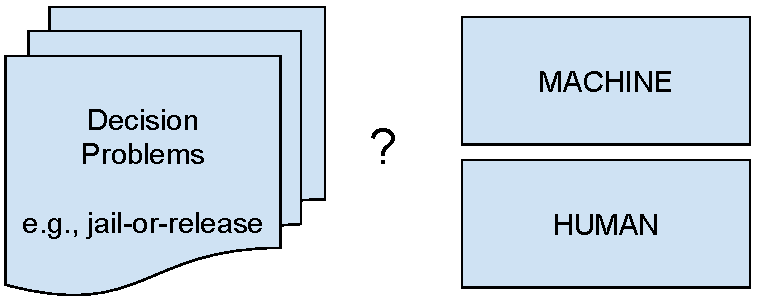
\includegraphics[width=0.5\textwidth]{Figures/problem_statement.pdf}

\end{frame}

\begin{frame}{Algorithmic Risk Assessment}
\begin{itemize}
\setlength\itemsep{5pt}%

\item + Human remains the upper hand and makes the final decision
\item + Clear responsibility

\item -- What about fairness?
\item -- How is the human influenced by the machine prediction?
\end{itemize}

\begin{figure}[t!]
    \centering
        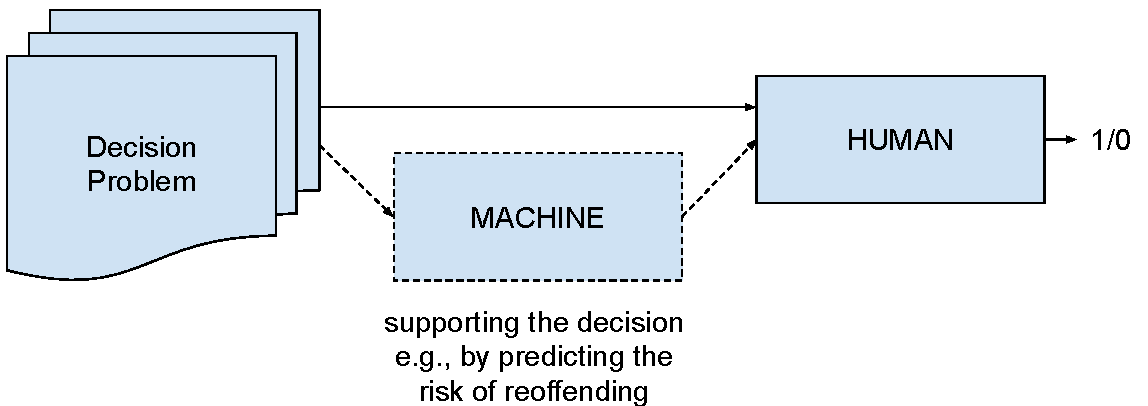
\includegraphics[width=0.8\textwidth]{Figures/human_decision.pdf}
\end{figure}
\end{frame}


\begin{frame}{How are Humans Influenced by Algorithmic Risk Prediction?}
\begin{itemize}
	\item Experiment on 500 pre-trial cases with known ground truth $y$
	\item Treatment group w/ algorithmic assessment ($N=6250$)
	\item Control group w/o algorithmic assessment ($N=7600$)
	\item Entry and exit survey 
\end{itemize}
\begin{figure}[t!]
	\centering
	\footnotesize
	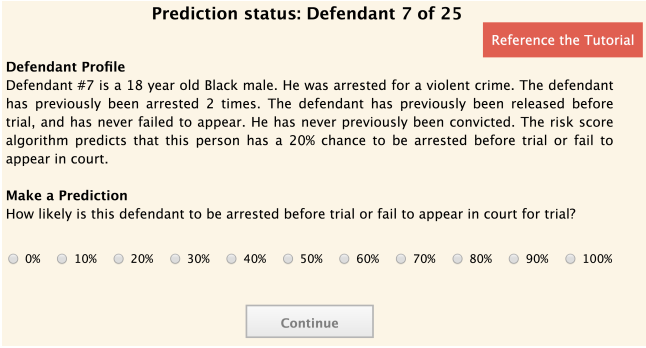
\includegraphics[width=0.7\textwidth]{Figures/experimentscreen.png}
	\caption{Amazon Turk experiment by \cite{green2019disparate}}
\end{figure}
\end{frame}

\begin{frame}{Hypothesis}
\begin{itemize}
	\item \textbf{H1 (Performance): }Participants presented with a
	risk assessment will make predictions that are less accurate
	than the risk assessment’s.
	\item \textbf{H2 (Evaluation): }Participants will be unable to accurately evaluate their own and the algorithm’s performance.
	\item \textbf{H3 (Bias): }As they interact with the risk assessment, participants will be disproportionately likely to increase risk predictions about black defendants and to decrease risk predictions about white defendants.
\end{itemize}
\end{frame}


\begin{frame}{Evaluation}
\begin{itemize}
	\item Reward: $r = [1-(\text{prediction}-\text{outcome})^2]$\\
	\item Risk-score influence on defendant $j$: $$I_j = \frac{t_j - c_j}{r_j - c_j}$$
	\item Influence of risk assessment on participant $k$ is: $$I^k = \frac{1}{25}\sum^{25}_{i=1}\frac{p_i^k -c_i}{r_i-c_i}$$
\end{itemize}
{\footnotesize
$r_j \ldots$ prediction made by risk assessment 

$t_j \ldots$ avg. prediction of treatment group on defendant $j$ 

$c_j \ldots$ avg. prediction of control group on defendant $j$ 

$p_i^k \ldots$ prediction of participant $k$ on defendant $j$ 


}

\end{frame}


\begin{frame}{Performance under Risk Assessment}
\begin{table}[]
	\begin{tabular}{@{}lll}
		\toprule
		& \textbf{Control} & \textbf{Treatment} \\ \midrule
		Average reward      & 0,756            & 0,786               \\ \midrule
		False positive rate & 17.7\%           & 14.8\%              \\ \bottomrule
	\end{tabular}
\end{table}
\begin{itemize}
	\item Participants in the treatment group earned a 4.0\% larger average
	reward and a 16.4\% lower false positive rate than participants in the
	control group (both with $p < 10^{-5}$)
\end{itemize}
\end{frame}

\begin{frame}{Performance under Risk Assessment}
\begin{table}[]
	\begin{tabular}{@{}llll}
		\toprule
		& \textbf{Control} & \textbf{Treatment} &\textbf{Risk assessment} \\ \midrule
		Average reward      & 0,756            & 0,786 & 0.807               \\ \midrule
		False positive rate & 17.7\%           & 14.8\% & 10.1\%             \\ \bottomrule
	\end{tabular}
\end{table}
\begin{itemize}
	\item  Despite being presented with the risk assessment’s predictions, the treatment group achieved
	a 2.6\% lower average reward and a 46.5\% higher false positive rate
	than the risk assessment (both with $p < 10^{-8}$)
	\item  Only 23.7\% of participants in the treatment group earned a higher average reward than
	the risk assessment over the course of their trial
\end{itemize}
\end{frame}


\begin{frame}{Self Evaluation of Participants}
\begin{itemize}
	%\item Exit survey (confidence, accuracy of assessment, influence, fairness)
	\item The more confidence participants expressed in their predictions, the less well they actually performed ($p=0.0186$)
	\item No significant relationship between the participant's evaluation of the risk assessments accuracy and actual performance
	\item No significant relationship between actual and perceived fairness
	\item Participants could generally discern how strongly they were influenced by the risk assessment
\end{itemize}
\end{frame}

\begin{frame}{Influence of risk scores on defendants}
\begin{itemize}
\item When risk score was lower than the average prediction in control group ($r < c$):
\begin{itemize}
	\item Risk assessment's influence similar regardless of the race
\end{itemize}
\vspace{2pt}
\item When risk score was higher than the average prediction in control group ($r > c$):
\begin{itemize}
	\item 25.9\% stronger average influence on predictions about black defendants than on predictions about white defendants
	\item Risk assessment leads to larger increase in risk for black defendants
\end{itemize}
\end{itemize}
\end{frame}


\begin{frame}{Influence of risk scores on defendants}
\begin{figure}[t!]
	\centering
	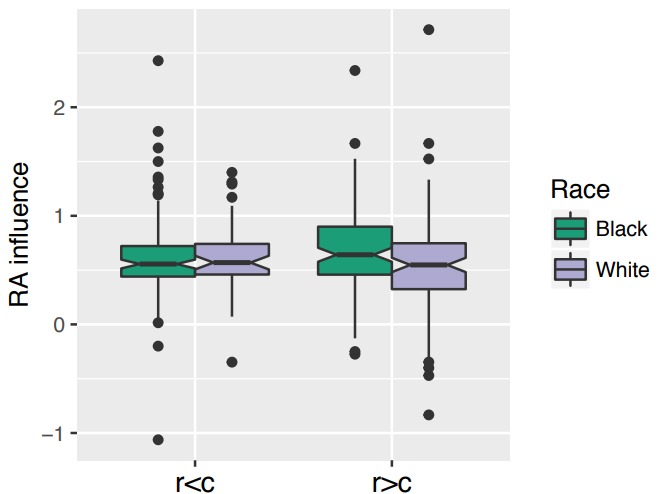
\includegraphics[width=0.8\textwidth]{Figures/influence_of_risk_score.png}
\end{figure}
\end{frame}



\begin{frame}{Limitations and Discussion}
\begin{itemize}
	\item Amazon Turk and no actual judges
	\item Only textual description, no face-to-face
	
	\item \TODO{todo}
	\item \TODO{todo}
\end{itemize}
\end{frame}

\begin{frame}{An alternative pattern: Learn to defer}
\begin{figure}[t!]
	\centering
	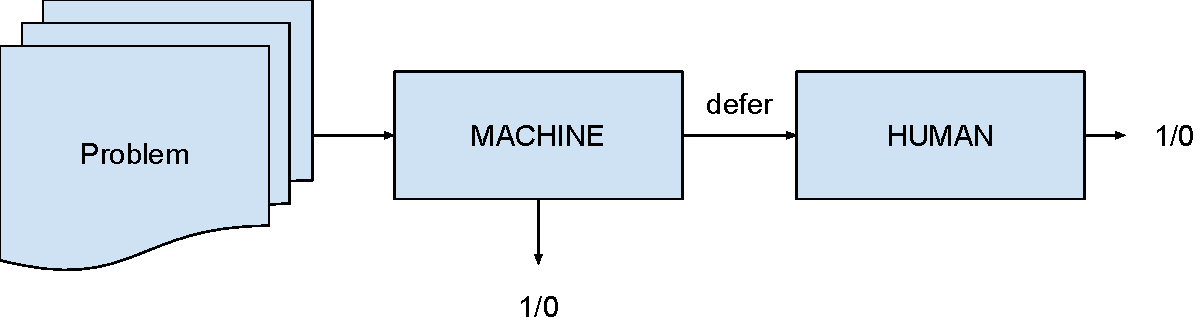
\includegraphics[width=0.8\textwidth]{Figures/defect.pdf}
\end{figure}
\end{frame}


\begin{frame}{Paper 1}
\end{frame}

\begin{frame}{Paper 1}
\end{frame}


\begin{frame}{Paper 1}
\end{frame}


\begin{frame}{Paper 1}
\end{frame}


\begin{frame}{Alternative pattern: Problem matching}
	\centering
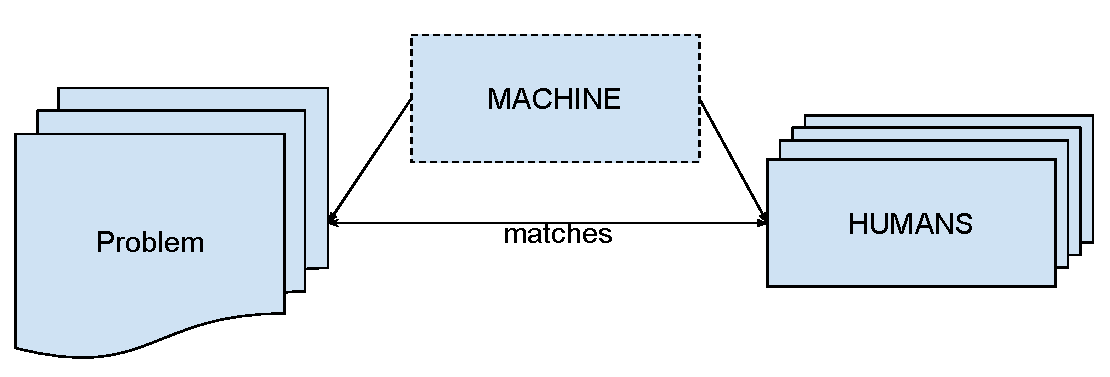
\includegraphics[width=0.8\textwidth]{Figures/matching.pdf}
\end{frame}


\begin{frame}{Paper 2}
\end{frame}

\begin{frame}{Paper 2}
\end{frame}


\begin{frame}{Paper 2}
\end{frame}


\begin{frame}{Paper 2}
\end{frame}

\begin{frame}{Conclusion}
\begin{table}[]
	\begin{tabular}{cl}
		\multirow{3}{*}{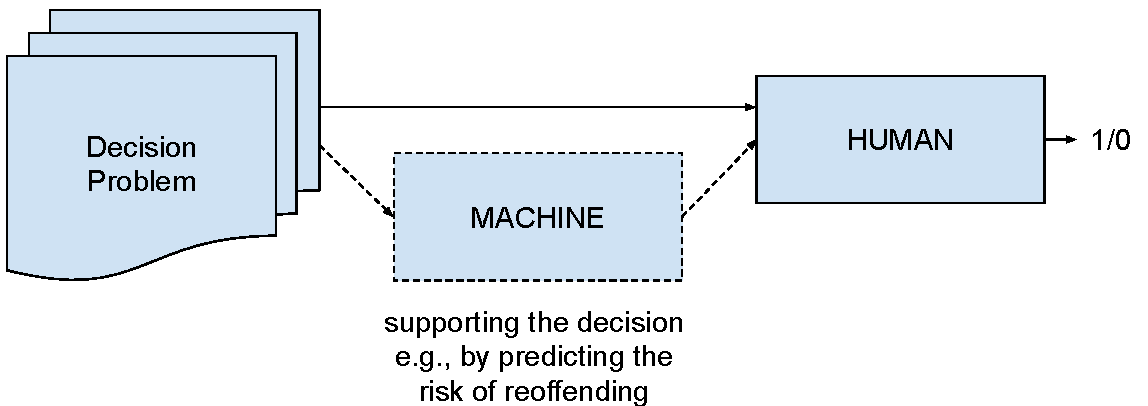
\includegraphics[width=0.4\textwidth]{Figures/human_decision.pdf}}&   + Benefit 1 		 \\
		& + Benefit 2\\
		& -- Disadvantage 1\\ 
		&\\
		\hline
		&\\
		\multirow{3}{*}{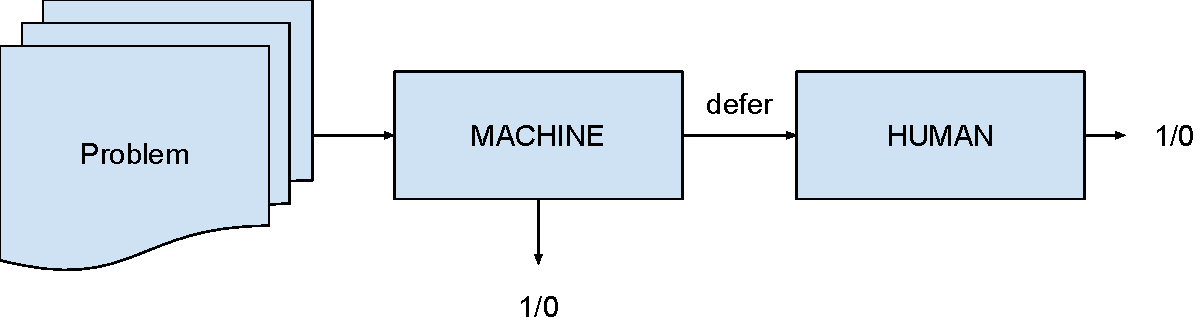
\includegraphics[width=0.4\textwidth]{Figures/defect.pdf}}&   	+ Text			\\
		& -- Lorem \\
		& -- Ipso \\
		&\\
		\hline
		&\\
		\multirow{3}{*}{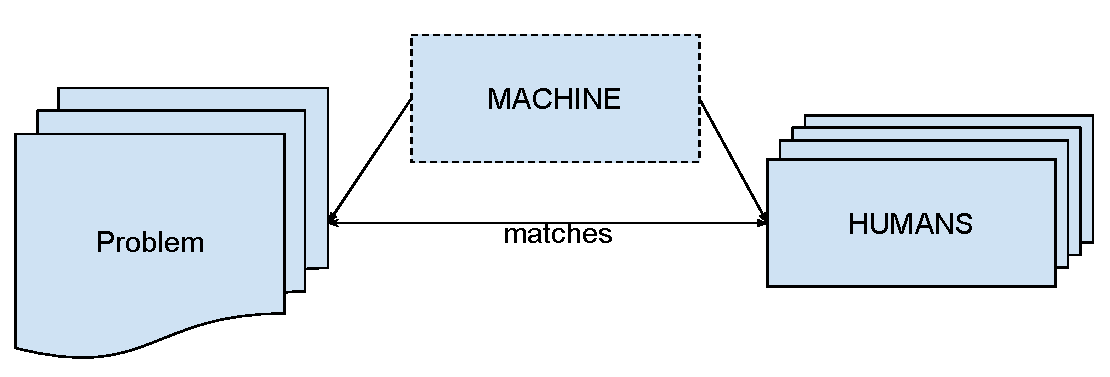
\includegraphics[width=0.4\textwidth]{Figures/matching.pdf}}&   + Dolor				\\
		& + More \\
		& -- Text \\
	\end{tabular}
\end{table}
\end{frame}

\begin{frame}{Other patterns worth mentioning}
\end{frame}

\begin{frame}{References}
\bibliography{Slides}
\bibliographystyle{apalike}
\end{frame}

\end{document}
